% !TEX root = ../thesis-example.tex
%
\chapter{Algorytmy korejestracji przestrzennej obrazów OCT}
\label{sec:algorytmy_korejestracji}

\textbf{Mozaiką} nazywamy obraz, który powstaje poprzez połączenie grupy obrazów zwanych kafelkami na podstawie ich wzajemnych relacji. Znanym oraz popularnym przykładem łączenia obrazów w jeden większy jest funkcja panoramy w telefonach komórkowych, czy aparatach fotograficznych. Od strony użytkownika proces tworzenia panoramy polega na powolnym przesuwaniu telefonem po linii poziomej do momentu aż żądany krajobraz zostanie uchwycony. Od strony urządzenia proces polega na wykonywaniu serii zdjęć oraz następnie łączenie nachodzących klatek w jeden obraz. Rezultatem jest jednolita panorama, która składa się z grupy mniejszych węższych zdjęć.

W niniejszej pracy celem jest stworzenie mozaiki OCT (przykład na rysunku \ref{fig:algorytmy_korejestracji:mosaic}), która powstaje z połączenia angiograficznych obrazów OCT (przykład obrazu angiograficznego OCT znajduje się z prawej strony na rysunku \ref{fig:obrazowanie_oct:bscan_vessels}).

\begin{figure}[H]
  \centering
  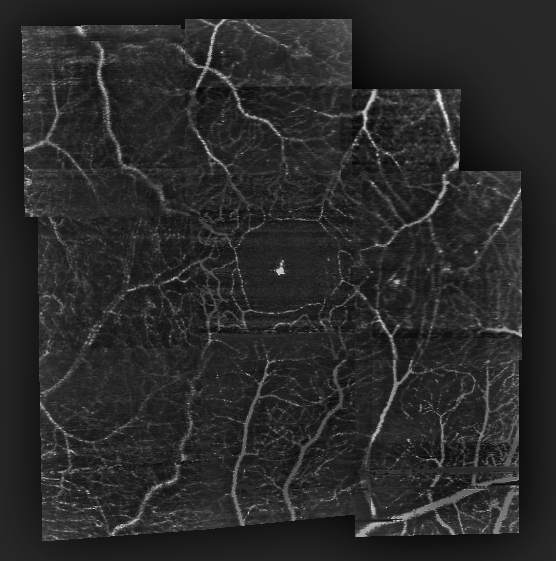
\includegraphics[width=10cm]{gfx/mosaic}
  \caption{Mozaika OCT stworzona z połączenia angiograficznych obrazów OCT.}
  \label{fig:algorytmy_korejestracji:mosaic}
\end{figure}

Proces automatycznego stworzenia mozaiki takiej jak na rysunku \ref{fig:algorytmy_korejestracji:mosaic} jest zadaniem nietrywialnym i wymaga dokładnej analizy wiedzy dziedzinowej oraz precyzyjnego wyboru metod. Pierwszym krokiem jest wybór modelu deformacji kafelek (sekcja \ref{sec:algorytmy_korejestracji:model_deformacji}), następnym etapem, który jest jednocześnie najbardziej wymagającym jest wybór metody wzajemnej korejestracji kafelek (sekcja \ref{sec:algorytmy_korejestracji:korejestracja_kafelek}). Posiadając zdefiniowane wzajemne relacje kafelek oraz ich docelowe położenie w finalnej mozaice należy wykonać proces łączenia kafelek (sekcja \ref{sec:algorytmy_korejestracji:laczenie_kafelek}). W każdej z tych sekcji została wyjaśniona idea metody w kontekście stworzenia mozaiki OCT, natomiast szczegółowy opis zaimplementowanych metod znajduje się w rozdziale \ref{sec:proponowane_algorytmy}.

\section{Model deformacji kafelek}
\label{sec:algorytmy_korejestracji:model_deformacji}

Model deformacji kafelek określa dozwolone przekształcenia geometryczne, które odwzorują piksele kafelka do pikseli kafelka w finalnej mozaice. Ze względu na to, że angiograficzne obrazy OCT znajdują się na jednej płaszczyźnie możliwy zbiór modeli deformacji ogranicza nam się do transformacji dwuwymiarowych, które zostały zobrazowane na rysunku \ref{fig:algorytmy_korejestracji:trans}.

\begin{figure}[H]
  \centering
  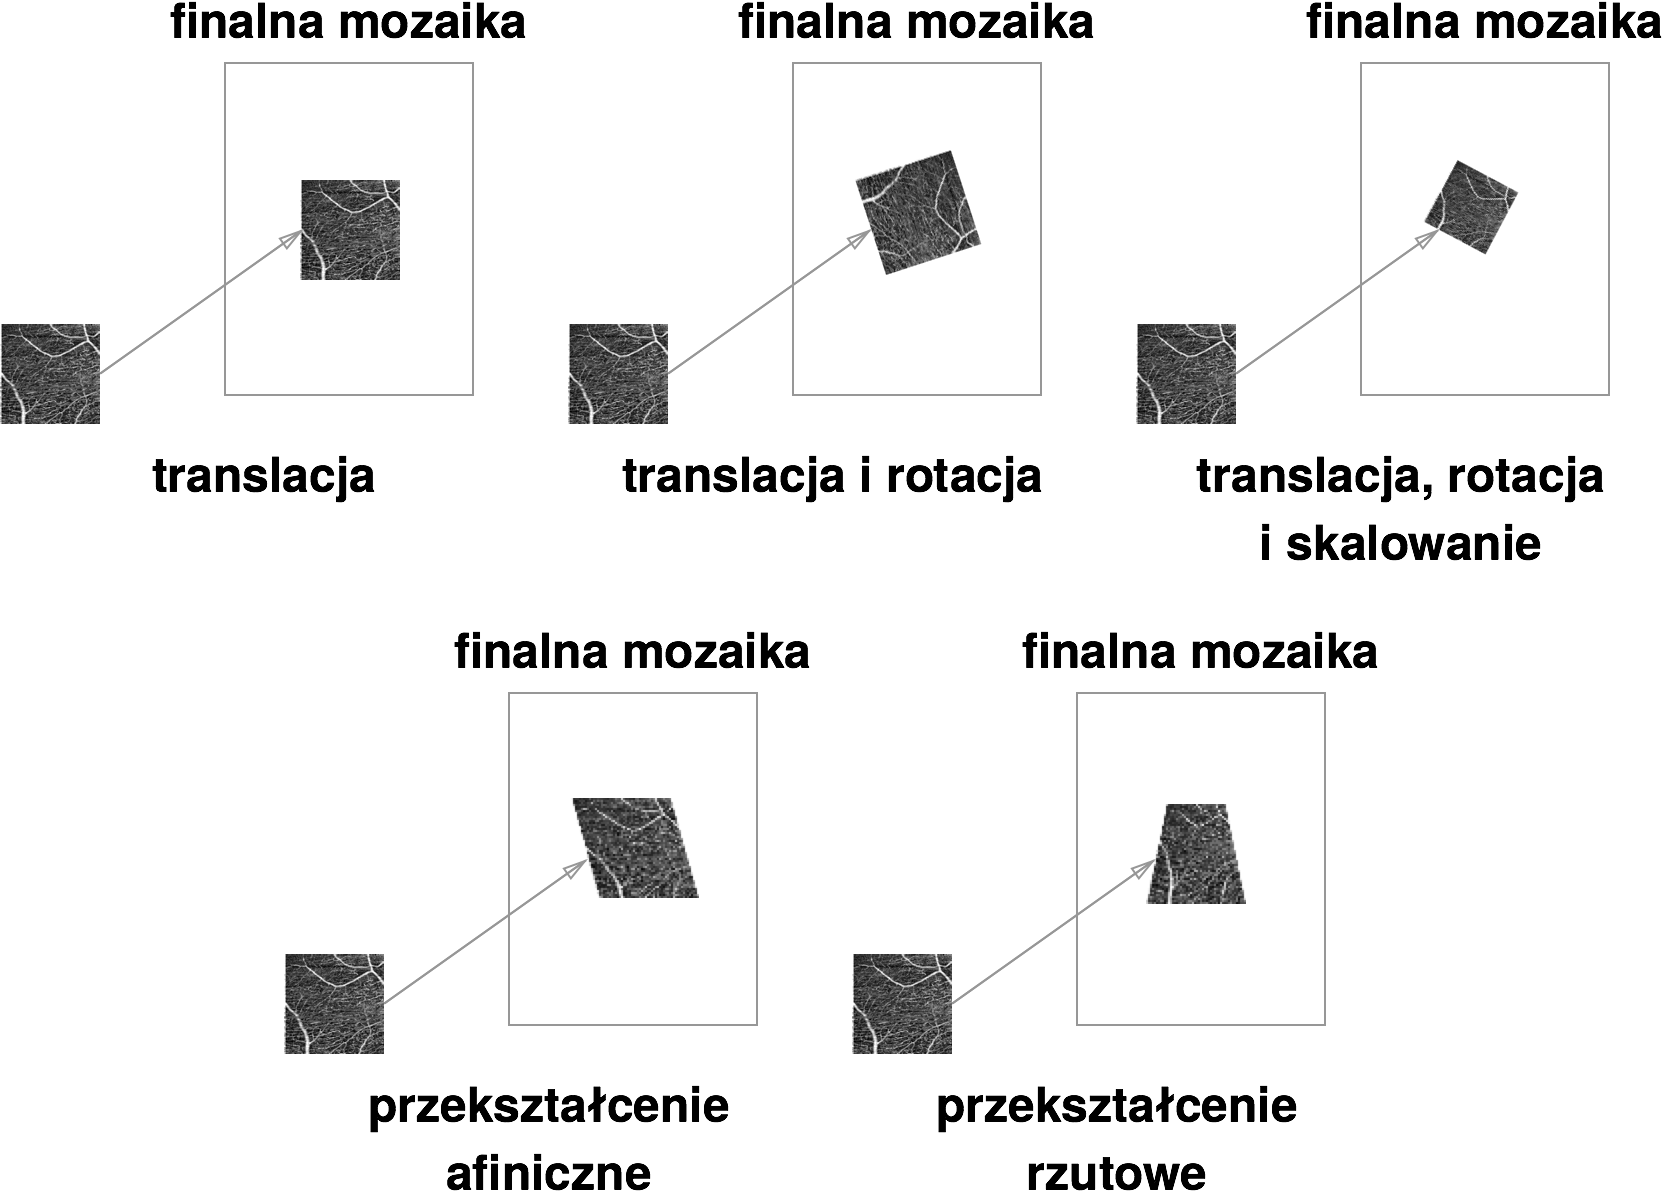
\includegraphics[width=\textwidth]{gfx/trans}
  \caption{Zbiór transformacji dwuwymiarowych dla przykładowego angiograficznego obrazu OCT.}
  \label{fig:algorytmy_korejestracji:trans}
\end{figure}

Idealnie OCT powinno tworzyć angiograficzne obrazy, które są względem siebie tylko przesunięte, natomiast w rzeczywistości pojawiają się zniekształcenia wynikające z niedokładności urządzenia oraz ruchu oka pacjenta, przez co niektóre kafelki są nieznacznie obrócone względem siebie. Z tego względu wybranym modelem deformacji kafelek został \textbf{model transformacji ciała sztywnego}, czyli połączenie translacji i rotacji.

\section{Korejestracja kafelek}
\label{sec:algorytmy_korejestracji:korejestracja_kafelek}

\section{Łączenie kafelek}
\label{sec:algorytmy_korejestracji:laczenie_kafelek}






















